
We developed a compiler and a virtual machine that runs
byte-code. The virtual machine for multicores makes use of the pthreads library.

\subsection{Overview}

The goal of our system is to keep the threads as busy as possible and to reduce inter-thread communication.
The load balancing aspect of the system is performed by our work scheduler that is based on a work
stealing algorithm. More specifically, threads can steal nodes of other threads to keep themselves busy.
Reduction of inter-thread communication is achieved by using a breadth-first search method to order nodes.

When the virtual machine starts, it reads the byte-code file and starts all threads.
As a first step, all threads will grab their nodes and assign the \texttt{owner} property of each node.
Because only one thread is allowed to do computation on the node at any giving time, this node's property
defines the thread with such permissions.
Next, we fill up the \emph{work queue} with the nodes we have picked. This queue
maintains the nodes that have new facts that need to be processed.

When a node sends a fact to another node, we need to check if the target node is not in the work queue of the owner thread.
If both nodes are in different threads, then we have a point of synchronization. At some point,
there will be no more work to do and the threads will go idle. There is a global atomic counter, a global
boolean flag and one boolean flag (active/idle) for each thread that are used to detect termination.
Once a thread goes idle, it decrements the global counter and changes its flag to idle. If the counter
goes to zero, the global flag is set to idle. Since every thread will be busy-waiting and checking
the global flag, they will detect the change and exit the program.

\subsection{Threads}

The work queue is actually implemented as two queues. First, there's one double-linked list for nodes
with priority equal to 0 called the \emph{normal queue}.
We use a double-linked list because it will be easier to move the node from this queue to the
\emph{priority queue}. The priority queue is an array based binary heap data structure that contains
all the unprocessed nodes with priority. To reduce the memory footprint of our queues, all the bookkeeping fields
such as the \texttt{next} and \texttt{prev} are part of the node data structure.
Each node also contains flags that indicate the queue where they are currently in and if they have facts to process.

\subsection{Nodes}

\begin{figure}[h!]
     \centering
   \resizebox{6cm}{!}{

    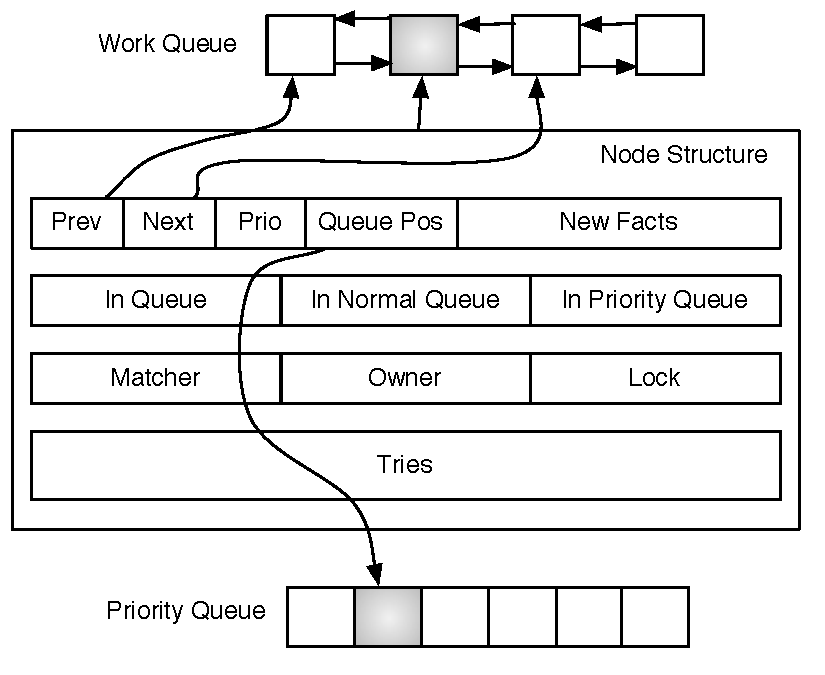
\includegraphics[width=0.5\textwidth]{node.pdf}}
    \caption{The node data structure.}
    \label{fig:node}
\end{figure}

The node data structure with an empty database occupies around 150 bytes.
In Fig.~\ref{fig:node} we present the node data structure and its fields. We summarize the data below:

\begin{description}
   \item[queue data]: Includes the field \texttt{Prev} (for the normal queue), \texttt{Next} (for the normal queue), \texttt{Prio} (priority) and \texttt{Queue Pos} (for the priority queue).
   \item[flags]: If the node is currently in the queue and in which queue. Includes \texttt{In Queue}, \texttt{In Normal Queue} and \texttt{In Priority Queue}.
   \item[temporary store]: A simple linked-list containing the unprocessed facts called \texttt{Temporary Store}.
   \item[database]: All the facts already processed which are true for this node. Is implemented as a trie and it is called \texttt{Tries}.
   \item[rule matcher]: The \texttt{Matcher} maintains the number of facts per predicate and which rules can be activated next. This is used for selecting the candidate rules.
   \item[owner]: Pointer to the owner thread. \texttt{Owner} in the figure.
   \item[lock]: A \texttt{Lock} mutex used to manipulate the node.
\end{description}

\subsection{Work Stealing}

When a thread runs out of nodes to process, it will pick a thread at random and try to steal one node
from the target thread. The stealer thread will pop a node from either the priority queue or the normal queue. We use locks for mutual exclusion when dealing with those queues. Note that when a
node is stolen, its owner information also changes to the stealer thread.

It is important to note that whenever a node sends a coordination action fact to a node in another thread, the fact is ignored, due to the costs of sending
coordination data between threads. We intend to design an efficient mechanism to solve this problem.

\subsection{Database}

The node database is implemented using the trie data structure. Tries are trees where facts are indexed
by the common prefix. Because we need to delete facts from the database, we implement each trie level
as a double linked list so trie nodes can be easily removed. If a trie level has too many nodes, we
transform the linked list into a hash table in order to improve lookup.

Each node uses a trie per predicate to store facts. During evaluation of rule bodies, we build a
\emph{match object}, which matches some arguments of the target predicate to instantiated values, so
that by searching the predicate trie from top to bottom, we can easily discard invalid trie branches.
